% !TeX root = ../../../book.tex

\subsection{更多示例}

现在我们已经掌握了这两个定理,让我们通过一些关系的例子来进一步理解它们。对于每个例子,我们将尝试判断它是否是等价关系。如果是,我们可以描述它的等价类。如果不是,我们可以参考其中一个定理,看看为什么它不是等价关系。\\

\begin{example}
    我们先从一个简单的例子开始。回顾一下我们在示例 \ref{ex:example6.2.9} 中定义的等式关系。我们已经解释过,``$=$'' 在任何集合上都是等价关系。具体来说,它将一个集合划分为等价类,而这些等价类正是集合的各个元素本身。例如,在集合 $\mathbb{N}$ 中,$[1]_{=} = \{1\}, [2]_{=} = \{2\}$,以此类推。所有的等价类都是\emph{单例的}(集合只有一个元素)。
\end{example}

\begin{example}
    我们再来看一个相对简单的例子。回顾一下我们在示例 \ref{ex:example6.2.5} 中定义的 $\mathbb{Z}$ 集合上的奇偶关系。这是一个等价关系,现在让我们来证明这一点。
    \begin{proof}
        设 $a, b, c \in \mathbb{Z}$ 是任意的。

        首先,不难发现 $(a,a) \in R$ 因为 $a$ 与其自身有相同的奇偶性。因此 $R$ 具有自反性。

        其次,假设 $(a,b) \in R$,所以 $a$ 和 $b$ 具有相同的奇偶性。那么显然 $b$ 和 $a$ 也具有相同的奇偶性,所以 $(b,a) \in R$。因此 $R$ 具有对称性。

        最后,假设 $(a,b) \in R$ 且 $(b,c) \in R$。如果 $a$ 是奇数,我们可以推导出 $b$ 为奇数且 $c$ 也为奇数;同理,如果 $a$ 为偶数,我们可以推导出 $b$ 为偶数且 $c$ 也为偶数。无论是哪种情况,$a$ 和 $c$ 都具有相同的奇偶性,所以必然有 $(a,c) \in R$。因此 $R$ 具有传递性。

        因为 $R$ 具有自反性、对称性和传递性,所以 $R$ 是一个等价关系。
    \end{proof}

    这意味着等价类集合 $\mathbb{Z}/R$ 构成 $\mathbb{Z}$ 的划分。现在让我们来确定该划分。

    考虑 $[0]_R$,这是所有与 $0$ 奇偶性相同的整数集合,即所有\emph{偶数}。因此,在这种情况下,
    \[\mathbb{Z}/R = \{O_{\mathbb{Z}}, E_{\mathbb{Z}}\}\]
    其中 $O_{\mathbb{Z}}$ 是奇数集,$E_{\mathbb{Z}}$ 是偶数集。这两个等价类都是无穷大的。
\end{example}

\begin{example}
    回顾我们在示例 \ref{ex:example6.2.6} 中定义的 $\mathbb{R}$ 上的顺序关系。这个关系是等价关系吗?我们可以通过检查定义中的每个属性来确定。要注意的是,无论 $x$ 是什么,只要 $x \in \mathbb{R}$,就有 $(x, x) \notin R$,因为 $x \nless x$。因此,$R$ 不具有自反性,所以它不是等价关系。(另外,$R$ 也不具有对称性,但它具有传递性。)

    为什么严格的顺序关系不会是等价关系呢?为什么我们希望等价关系是自反的?想想\emph{等价类}的概念;等价关系应该把整个集合的元素划分成几部分,我们可以通过属于某部分的一个元素来识别这部分。对于非自反的关系,有些元素不属于它们自己的``等价类'',这显然是不理想的!

    (后续问题:对于自反的顺序关系 $\le$,它是等价关系吗?为什么是或者为什么不是?)
    
    换句话说,$\mathbb{R}$ 上的 ``$<$'' 关系并没有把实数划分为几部分。基于这一点,并结合定理 \ref{theorem6.4.10} 的\emph{逆否}命题,我们可以得出 ``$<$'' \emph{不是}一个等价关系。
\end{example}

\begin{example}
    定义 $\mathbb{R} \times \mathbb{R}$ 上的关系 $\sim$ 为
    \[(x, y) \sim (u, v) \iff x \le u \land y \le v\]
    即使不检查其具体属性,我们也可以尝试判断它是否是等价关系。为此,我们选取集合中的一个特定元素,并查看与该特定元素相关的所有元素。在下图中,我们使用 $(1, 1)$ 作为这个特定元素。

    \begin{center}
        {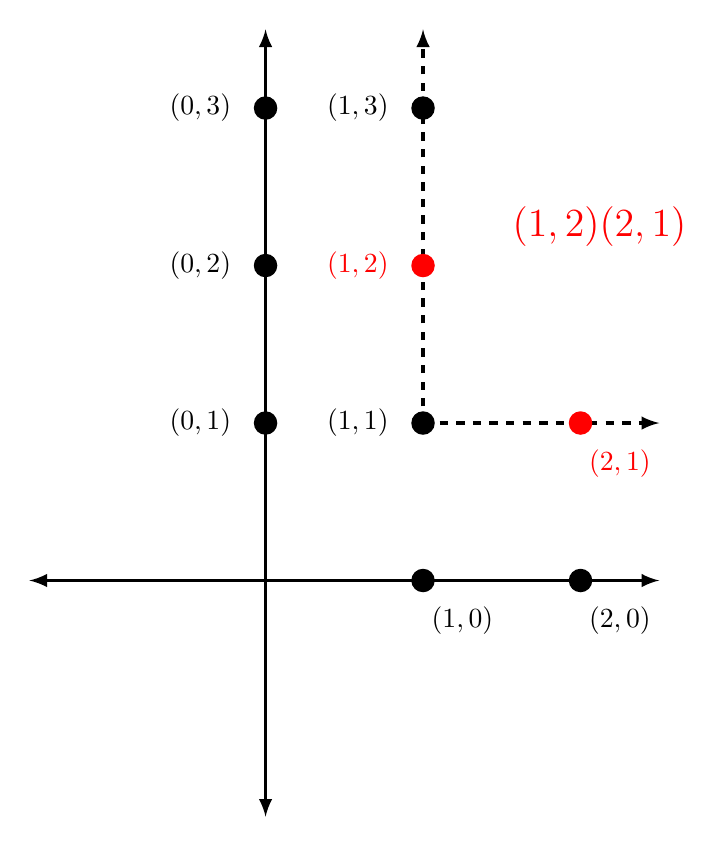
\begin{tikzpicture}[very thick,scale=2]
            \draw[latex-latex] (-1.5,0) -- (2.5,0); 
            \draw[latex-latex] (0,-1.5) -- (0,3.5); 
            \foreach \x in  {1,2}
            {
                \node at (\x, 0)[circle,fill,inner sep=3pt]{};
                \draw[shift={(\x+0.25,-0.1)}] node[below] {$(\x, 0)$};
                
            }
            \foreach \y in  {1,2,3}
            {
                \node at (0, \y)[circle,fill,inner sep=3pt]{};
                \draw[shift={(-0.15, \y)}] node[left] {$(0, \y)$};
            }
    
            \draw[dashed,-latex] (1,1) -- (2.5,1); 
            \draw[dashed,-latex] (1,1) -- (1,3.5); 
            \foreach \y in  {1,3}
            {
                \node at (1, \y)[circle,fill,inner sep=3pt]{};
                \draw[shift={(0.85, \y)}] node[left] {$(1, \y)$};
            }
    
            \node[red] at (1, 2)[circle,fill,inner sep=3pt]{};
            \draw[color=red, shift={(0.85, 2)}] node[left] {$(1, 2)$};
            \node[red] at (2, 1)[circle,fill,inner sep=3pt]{};
            \draw[color=red, shift={(2.25, 0.9)}] node[below] {$(2, 1)$};
    
            \draw[color=red, font=\Large, shift={(1.5, 2.25)}] node[right] {$(1,2) \nsim (2,1)$};
        \end{tikzpicture}}
    \end{center}

    请注意,$\sim$ 的定义条件要求一个点必须位于另一个点的``右上方''才能使两者相关。同时,不等式是``$\le$'',因此第二个点不必\emph{严格}位于上方或右侧。

    因此,我们可以从上图看到,$(1, 2) \sim (1, 1)$(因为 $1 \le 1$ 且 $1 \le 2$)。同理,$(1, 1) \sim (2, 1)$。因此,点 $(1, 2)$ 和 $(2, 1)$ 都与 $(1, 1)$ 相关。为了使 $\sim$ 成为\emph{等价关系},我们需要 $(2, 1$) 和 $(1, 2)$ 也彼此相关。因为它们必须同属于 $(1, 1)$ 的``等价类''。然而,遗憾的是,$(1, 2) \nsim (2, 1)$。第二个点严格位于第一个点的``左下方'',因此不满足 $\sim$ 的定义条件。

    这意味着所有与 $(1, 1)$ 相关的元素的集合\textbf{不能}形成一个``封闭集合''。从数学上讲,这些元素的集合不是一个等价类。因此,$\sim$ \textbf{不是}一个等价关系。

    现在,试着识别 $\sim$ 具有哪些性质和不具备哪些性质。它具有自反性吗?具有对称性吗?具有传递性吗?为什么具有或者为什么不具有?通过这样做,你会再次证明 $\sim$ 不是一个等价关系。事先弄清楚这一点,是不是很有帮助呢?我们建议,当你遇到一个定义好的关系时,可以做类似的分析。你能找出``等价类''可能是什么吗?如果能,那么你对这个关系为何以及如何是等价关系有了一些直觉,这将帮助你描述等价类。如果不能,那么你也会对如何反驳这种说法有一些理解。
\end{example}

\subsubsection*{[选学] $\mathbb{Z}$ 是如何从 $\mathbb{N} \times \mathbb{N}$ 上的等价关系生成的}

还记得第 \ref{ch:chapter03} 章中的那个复杂习题吗?它要求你证明某些关于自然数对的性质,并声称这是在证明整数的存在性。那到底是怎么回事呢?现在回头看看习题 \ref{exc:exercises3.11.22}。你会发现问题的最后三个部分要求你证明我们定义的集合 $R$ 是集合 $P$ 上的\textbf{等价关系}(底层集合是 $P = \mathbb{N} \times \mathbb{N}$)。好好看一下!你已经证明了 $R$ 具有自反性、对称性和传递性。

这个练习表明(在这里我们略过了一些细节)任何负整数都可以表示为两个整数之差为该负整数的\textbf{等价类}。也就是说
\[-1 \;\text{``$=$''}\; [(1, 2)]_R = \{(1, 2),(2, 3),(3, 4), \dots \}\]
再比如
\[-3 \;\text{``$=$''}\; [(1, 4)]_R = \{(1, 4),(2, 5),(3, 6), \dots \}\]
这只是一个直观的解释,从数学上讲并不严格,但这就是主要思路!
